\documentclass[11pt]{article}
\usepackage{ctable,microtype,natbib,amsmath,amssymb,fullpage,graphicx,tabularx}
\usepackage{siunitx}
\usepackage{cleveref}
\usepackage{keyval,kvoptions,fancyvrb,float,ifthen,calc,ifplatform,pdftexcmds,etoolbox,lineno}
\usepackage[utf8]{inputenc}
\usepackage{color}
\usepackage[danish]{babel}
\usepackage[left=25mm, right=25mm, top=25mm, bottom=25mm]{geometry}
\usepackage{lastpage}
\usepackage{amsthm}
\setlength\parindent{0pt}
\usepackage{fancyhdr}
\usepackage{dcolumn}
\usepackage{minted} 
\usepackage{setspace}
\onehalfspacing

\title{hahahaahah grimme}
\author{Christian Bondesen - 201511621}

\begin{document}
\maketitle
%-----------------------------------------------------------------------------------
%------------------------------------Hardware Analyse-------------------------------
%-----------------------------------------------------------------------------------
\section{Analyse af hardwaredele}
I følgende sektion gennemgås der tanker der er udtænkt da udarbejdelsen af hardwaren skulle gennemføres. Der vil blive beskrevet nogle detaljeret design for forskellige hardwaredele, som tager udgangspunkt i specifikationen og arkitekturen. Hvis man ønsker mere information i forhold til implementeringen af hardwaren, henvises der til projektdokumentation(mangler ref).

\subsection*{Hardware analyse}
I start forløbet af projektet blev der udtænkt nogle tanker om hvilke bestanddele hardwaren skulle bestå af. Tanken er at der dannes et overordnet system ved navn Smart Morning System (SMS), der skulle bestå af forskellige hardwaredele. Figur \ref{fig:overvejelserBDD} viser en BDD af de første overvejelser. 

	\begin{figure}[!ht]
	 	\centering
	 	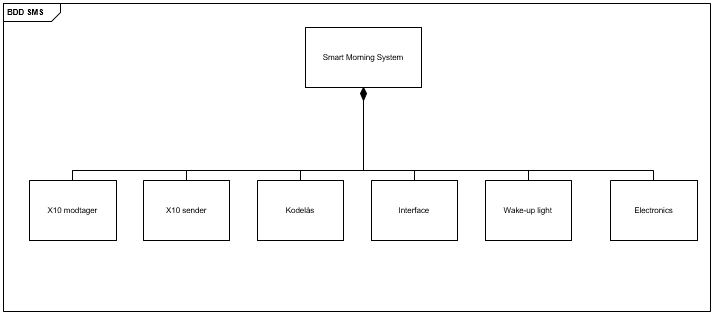
\includegraphics[scale = 0.8]{BDD-overvejelser-SMS}
	 	\caption{BDD over de første overvejelser for designet}
	 	\label{fig:overvejelserBDD}
	 \end{figure} 

Efter udarbejdelsen af dette diagram er det muligt at nedbryde disse blokke for at beskriver grænseflader og skabe overblik over specifikke funktionaliteter for det blokkene.\\
Der er valgt i den endelige BDD ikke at have interface med da det ikke er et specifikt stykke hardware. Derudover er X-10 sender og modtager brudt yderligere ned, for at skabe overblik over de dele som de individuelt består af. Her henvises til System Arkitekturen i projektdokumentationen for yderligere information(mangler ref).

 \subsection*{Wake-up light}
 Der blev i starten af projektforløbet besluttet at der skulle være et bestemt lys der skulle hardcodes til vores system. Dvs. at man ikke kunne undgå denne funktion, da det er det som skulle være fundamentet for Smart Morning System. Dette lys skulle start med et svagt lys og derefter i løbet af nogle minutter stige i intensitet.\\
 Efterfølgende i projektforløbet blev det senere konkluderet at der ikke kunne findes overskydende tid til at samme sætte Wake-up light op. Derfor blev der i stedet har vi sat 14 LED'er op som, burde lyse den bit koden som er modtaget af systemet.

\subsection*{Tovejskommunikation}
I starten af projektforløbet var der tænkt at systemet skulle være tovejskommunikation. Dvs. det skulle være muligt for systemet at sende tilbage til computeren så brugeren kunne se at den har sendt alarmen til lyset eller den elektroniske enhed.\\
Efterfølgende i projektforløbet, blev det dog besluttet af gruppens medlemmer at forkaste denne funktionalitet for systemet, da det ville tage for lang tid at udtænke og gennemføre denne del.

\subsection*{Overvejelser til filtre}
Efter at have læst ``AN236 Application Note'' blev det meget hurtigt klart at en eller anden form for filtrering af signalerne da der sker en overlejring af to forskellige signaler. Der blev først overvejet et båndpasfilter til X-10 modtager da den udelukkende er 



\end{document} 
